\section{\label{sec:drill-deploy}Drilling and Deployment}

\subsection{\label{sec:hot_water_drilling}Hot Water Drilling}

Transforming a cubic kilometer of Antarctic ice into an astrophysical
particle detector required drilling 86 boreholes
approximately 60 cm in diameter to a depth of 2500~m. Hot water drilling
was the only
feasible technology to provide rapid access to the deep ice on this scale.
Instrumentation was deployed into the water-filled boreholes, becoming
frozen in place and optically
coupled with the surrounding ice sheet. The 5~MW Enhanced Hot Water Drill
(EHWD) was designed and built specifically for this task,
capable of producing the required boreholes at a maximum rate of one hole per 48
hours. This section contains an abbreviated description of the drill; a more detailed description
can be found in ref.~\cite{ehwd}.

The procedure involved a drilling phase to create the initial hole,
followed by an upward reaming phase to give the 
hole a targeted diameter profile.  During drilling, the location of
the drill was recorded with an onboard navigational pack consisting of
a Paroscientific pressure sensor
(model 8CB4000-I) to measure depth, two
liquid pendulums to measure tilt, and a fluxgate compass to measure
orientation. The hole diameter was larger than
the DOM (35~cm diameter) to compensate for closure from refreezing to provide sufficient
time to deploy instrumentation, with contingency time for delays.  The
elapsed duration from the end of drilling until the hole closes to
less than the DOM diameter is referred to as the hole lifetime. IceCube drilling was
completed in seven field seasons (approximately 21 months total time).
Peak performance occurred in the 2009--2010 season with 20 holes drilled
(early November to mid-January).  The drill specifications and performance
are shown in Table~\ref{tab:ehwd_system} and
Table~\ref{tab:ehwd_system_peak}. figure~\ref{fig:drilldepthtime} shows the
drilling and reaming time for a typical hole in the 2009--2010 season.

\vspace{\baselineskip}

\begin{minipage}{\textwidth}
  \centering \captionof{table}{EHWD System Characteristics}
  \begin{tabular}{ l  r }
 \hline
    Specification & Value \\ \hline Total Power (Thermal + Electrical)
    & 5 (4.7 + 0.3) MW \\ Maximum Drill Speed & 2.2 m/min \\ Maximum Ream
    Speed & 10 m/min \\ Water Flow (delivered to main hose) & 760 L/min
    \\ Water Temperature (delivered to main hose) & \SI{88}{\celsius}
    \\ Water Gauge Pressure (at main pumps) & 7600 kPa\\
 \hline
  \end{tabular} 
  \label{tab:ehwd_system}
\end{minipage}
\vspace{\baselineskip}

\begin{minipage}{\textwidth}
  \centering \captionof{table}{Average and peak performance for a 24-hour
    lifetime hole of 2500 m depth. Peak performance corresponds to
    string 32 from the 2009--2010 drilling season, which had the
    fastest drilling + reaming time.}
  \begin{tabular}{ l  r  r }
\hline
    Specification & Avg. Value & Peak Value\\ 
\hline 
Total Fuel\footnote{Total Fuel includes deep drilling/reaming and firn
      drilling}, AN-8 & 21,000 L & 15,000 L \\ Time to Drill/Ream & 30 hr&
    27 hr \\ Hole Production Cycle Time\footnote{Hole Production Cycle Time
      is the elapsed time from start of one hole to start of the next hole}
    & 48 hr & 32 hr \\
\hline
    \end{tabular}
  
  \label{tab:ehwd_system_peak}
\end{minipage}
\vspace{\baselineskip}

Hot water drilling was not practical in the firn layer, the 50~m-thick surface layer of
compressed snow above the ice, because the firn
absorbs hot water without melting a hole.  An independent
firn drill was designed that consisted of a conical drill
head wrapped in copper tubing through which hot water circulated at high speed,
melting the snow by contact. Hot water drilling commenced after the firn
drill completed the first portion of the hole. The firn drill had its own
water supply and heater in order to operate in parallel with hot water drilling
at other holes. The firn drill reliably achieved a rate of 2~m per hour~\cite{ehwd}.

\begin{figure}[!ht]
 \centering
 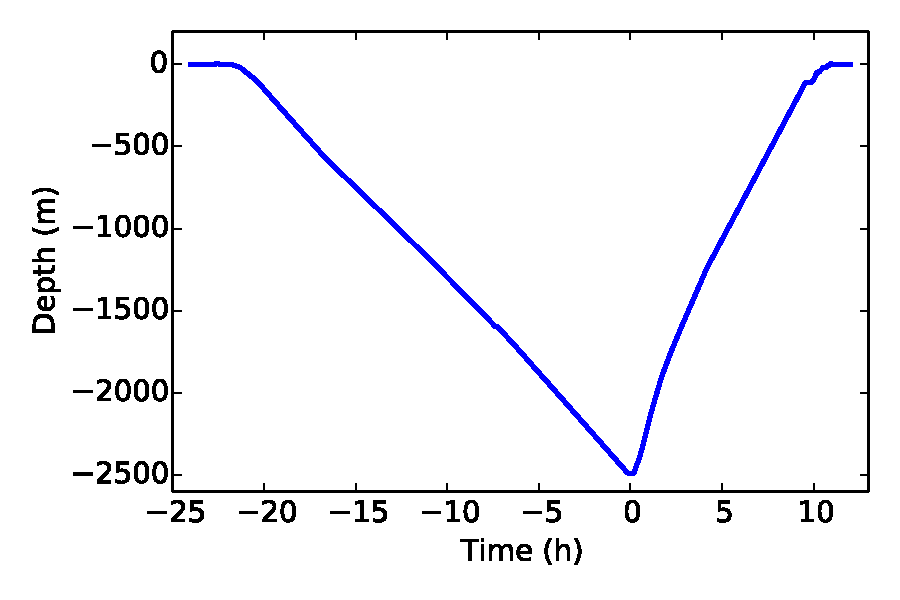
\includegraphics[width=0.7\textwidth]{graphics/drill/drill_depth_hole41.pdf}
\caption{Drilling and reaming profile for string 41, from the 2009--2010
  deployment season. Zero time is maximum drill depth, so drilling time is
  negative and reaming time is positive.}
\label{fig:drilldepthtime}
\end{figure}

The EHWD system was implemented across two separate sites. The Seasonal
Equipment Site (SES) provided electricity and a stable supply of hot
pressurized water, and the Tower Operations Site (TOS) was where the hole
was drilled.  The two sites were linked by long cables and insulated
hoses. The SES comprised generators, water tanks, pump and heating
buildings, a central control building, mechanical and electrical shops,
spare parts storage, and the Rodriguez well system (Rodwell), which
provides water to compensate for the volume change from ice to water
in each hole~\cite{rodriguez_well}. Hoses and cables connected SES subsystem buildings together, and
wherever necessary custom electrically heated hoses were installed,
providing an effective freeze mitigation strategy. The TOS included the
drill tower and attached operations building as well as the hose and cable
reels.  There were two towers and one set of drill reels.  After drilling,
drill reels were moved to the next hole location, where the second tower
had already been staged; the first tower stayed at its existing location
to support deployment of the instrumentation.  Once deployment had
finished, the first tower could be moved to the next location while
drilling at the second tower was underway.  This leapfrog sequence of the
tower structures reduced hole turnover time and allowed nearly
continuous drilling operations.

Due to the size and complexity of the SES, it remained stationary
throughout each drill season.  At the end of the drill season, the SES was
decommissioned and repositioned for the following drilling season.  The
distance between the SES and TOS had a practical limit, referred to as
reach, which defined the boundary of a seasonal drilling sector.  The
maximum reach
of the EHWD was 450~m, limited by pressure and voltage drop through the
SES--TOS link.

Each drilling season started with a staggered arrival of drill crew members
while the SES and TOS were excavated from accumulated snow drift and commissioned.  Season startup
tasks included SES and TOS warming and hookups, reinstallation of
do-not-freeze equipment (such as motor drives, sensors, and some
rubber items such as gaskets), generator commissioning, safety checkout and system
tuning, initial (``seed'') water delivery to begin the drilling process, and Rodwell development.  This phase typically
took four weeks.

The production drilling sequence was to drill, ream, and move to the next
location. The drill crews worked in three shifts per day of ten people
per shift. Independent firn drilling stayed ahead of deep drilling by at
least two holes, and often the Rodwell and first few holes of
the season had already been firn-drilled the prior season. Hole production rate was 48 hours per hole on average,
and the quickest cycle time was 32 hours. The idle phase
between holes was characterized by minimal flow through the
system and included regular maintenance tasks and deployment of IceCube
instrumentation.  

System shutdown would begin approximately two weeks before the end of the
austral summer season. Shutdown tasks included flushing the system with
propylene glycol, blowing out the plumbing with compressed air, removing
do-not-freeze equipment for warm storage, storing the TOS structures and
other support equipment, and finally, moving the SES into place for the
following season.  Due to a strong safety culture and retention of
experienced personnel, IceCube had only
four reportable drilling-related safety incidents in approximately 52 on-ice 
person-years. 

\subsection{\label{sec:deployment_inst}Deployment Procedures and Instrumentation}

DOM deployment required 60 DOMs staged in the drill tower, various
attachment hardware, pressure sensors, and the in-ice cable on a spool
outside the drill tower. The hole diameter was logged before deployment
using calipers on the drill head. After verification that the hole was 
ready for deployment and a pre-deployment safety check was carried out, the in-ice cable
was pulled over the top of the tower above the open hole. Four 100-pound
weights were connected together and attached via a 2.1~m steel cable to a
DOM that had a 17 meter penetrator assembly (see figure~\ref{fig:domcable}). The weights and
lowermost DOM were attached to the bottom of the in-ice cable via a 15.5~m
steel cable. After lowering of the DOM and weights, the next DOM with a
1.8~m penetrator assembly was attached to the in-ice cable. The two DOMs were
then electrically connected to the in-ice cable at the breakout. A
Paroscientific pressure sensor (model 8CB4000-I) was attached just above the second DOM
and a Keller AG pressure sensor (model 300DS-340-003700) was attached in the middle of the
instrumented section of the string. The
pressure sensors were read out during deployment to confirm that the string
was properly descending into the hole.   DOMs with 17~m and
1.8~m penetrator assemblies were alternately attached to the in-ice 
cable, until all 60 DOMs were attached, after which the remaining 1.5~km of
in-ice cable was lowered into the hole (the ``drop'' phase). The top of the
cable was secured by an anchor trenched into the snow near the hole. After the
cable was secure, its end was taken off of the spool and connected to the
Surface Junction Box (SJB). An example of the time profile of deployment from pressure sensor
attachment to string drop is shown in figure~\ref{fig:deploytime}.

\begin{figure}[!ht]
 \centering
 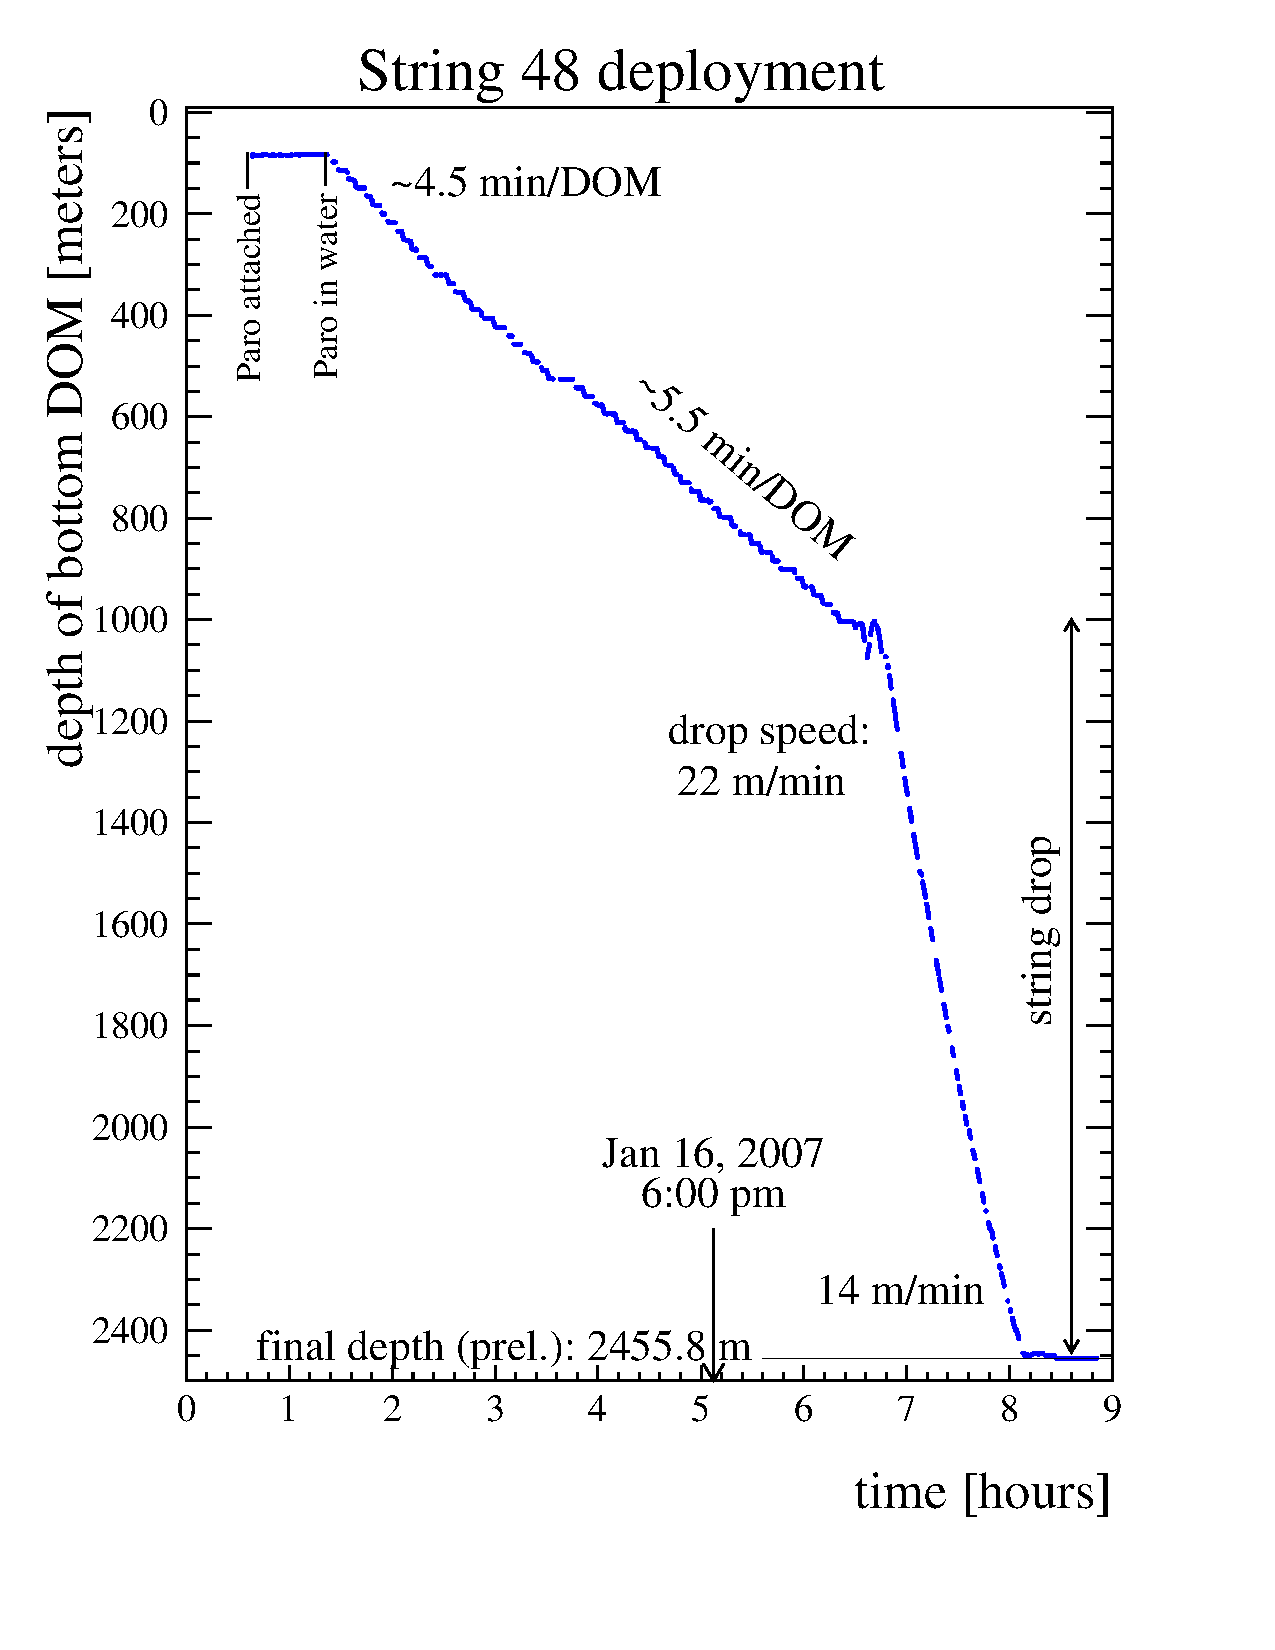
\includegraphics[width=0.70\textwidth]{graphics/drill/String48_deploy.pdf}
\caption{Depth of the lowermost DOM vs.~time for String 48, deployed in the
  2006--2007 season. The final depth is the preliminary Stage~1 depth
  measured during deployment (section~\ref{subsec:stage1_geo}),
prior to the Stage~2 corrections derived from LED flasher
measurements (section~\ref{subsec:stage2_geo}).}
\label{fig:deploytime}
\end{figure}

Dust loggers were deployed in selected holes in order to measure the
concentration of dust and volcanic ash as a function of depth at various
locations in the detector, a critical component of the overall measurement
of the optical properties of the
ice~\cite{Aartsen:2013rt,citeulike:2998650}. A dust logger consists of a 404~nm laser line source emitted horizontally in a
fan pattern, paired with an integrated
photomultiplier tube and digital photon counter for light
detection. Disposable dust loggers were deployed in two holes, and reusable dust loggers were
deployed in six holes. Each disposable dust
logger was attached to the main cable between the lowermost DOM and the
weight stack, and an extension cable ran between the dust logger and the
bottom breakout, just above the next-to-lowest DOM. In this mode, the hole
was logged once during deployment, and the logger was not
retrieved. The reusable dust logger was used to
log holes just before deployment, using a separate winch. The reusable
dust logger produced two logs for the 
hole, one in the up direction and one in the down direction, which were used for
reciprocal calibration.


\subsection{Geometry Measurement}

The geometry of the detector was determined using drill and survey data
during deployment (Stage 1), and then corrected and refined using the LED
flashers in ice (Stage 2). The IceCube coordinate system is
defined relative to the South Pole grid coordinate system (Northings and
Eastings) that moves with the ice sheet.  Elevation is defined relative to
Mean Sea Level.  The IceCube coordinate system origin
is located at 46500'E, 52200'N, at an elevation of 2900~ft (883.9
m).  This origin is located close to the center of the instrumented volume of
IceCube, about 2000~m below the surface of the ice. The $y$-axis of
the IceCube coordinate system is aligned with the Prime Meridian (Grid North),
pointing toward Greenwich, UK. The $x$-axis of the IceCube coordinate
system points 90$^{\circ}$ clockwise from the $y$-axis (Grid East). The $z$-axis is
normal to the Earth's surface, pointing upward. 

\subsubsection{\label{subsec:stage1_geo}Stage 1 Geometry Measurement}
The $(x,y)$-coordinates of the string were calculated using the position of
the drill tower. Before deployment, when the drill tower was in position, at
least three of the tower corners were surveyed from at least one control
point.  The coordinates for the center of the hole in the tower floor were
calculated from the corner coordinates. The string was assumed to be
vertical, so the $(x,y)$-coordinates from the tower were used at all
depths on the string. The drill
data show deviations of less than 1~m from vertical that are not
included in the detector geometry but have been validated
with flasher data for select strings, as discussed in section~\ref{sec:trilateration}. 

The depth of the lowest DOM on the string was calculated using pressure
readings from the pressure sensor, converted to depth by correcting for the
compressibility of the water in the hole and the ambient air pressure
measured before the pressure sensor enters the water. The distance from the
tower floor to the water surface was measured with a laser ranger
during deployment. The
vertical DOM spacings were also measured with a laser
ranger aimed down the hole after each DOM attachment. All depths were
converted to $z$-coordinates in the IceCube 
coordinate system.

\subsubsection{\label{subsec:stage2_geo}Stage 2 Geometry Measurement}

The LED flashers on the DOMs were used to correct the depths of the strings relative to
the Stage 1 geometry measurements. The correction was calculated by flashing
the horizontal LEDs on a DOM at the surrounding strings and finding the
leading edge of the time distribution of the light recorded by the
receiving DOM, denoted $t_0$. The distance corresponding to the leading
edge time is $d = c_{\mathrm{ice}} \cdot t_0$, and the distances for all receiving
DOMs are plotted as a function of the vertical distance between the flasher
and the receiver, $z' = z_{\mathrm{receiver}} - z_{\mathrm{flasher}}$. The resulting curve
describes a hyperbola, $d = \sqrt{D^2 + (z' -\Delta z)^2}$, where $D$ is
the horizontal distance between the flasher string and the receiver string,
calculated from Stage 1 data, and $\Delta z$ is the relative offset between
the depths of the flashing and receiving string as shown in
figure~\ref{fig:geohyperbola}. The hyperbolic fit was performed
simultaneously on multiple flasher--receiver pairs; in order to avoid
bias, this global fit was performed multiple times on randomly
selected sets of string pairs. An average offset was calculated for
each string and applied as a correction to the Stage~1 $z$-coordinates
of all DOMs on that string. The correction was typically less than 1~m
relative to the Stage 1 data, but could be as large as 20~m (larger than the
17~m DOM spacing) in cases where the pressure sensor failed during string
deployment before it recorded the final depth reading, resulting in a
poor estimate of the Stage~1 depth. The Stage 2 depth correction was less than 3~m for 93\%
of the strings. The uncertainty on the correction varied from string
to string but was typically less than 0.2~m. The uncertainty on the
absolute $z$-coordinate is 1~m, based on timing residual studies from
downgoing muons~\cite{IC3:perf}.

\begin{figure}[!ht]
  \captionsetup[subfigure]{labelformat=empty} \centering
  \subfloat[]{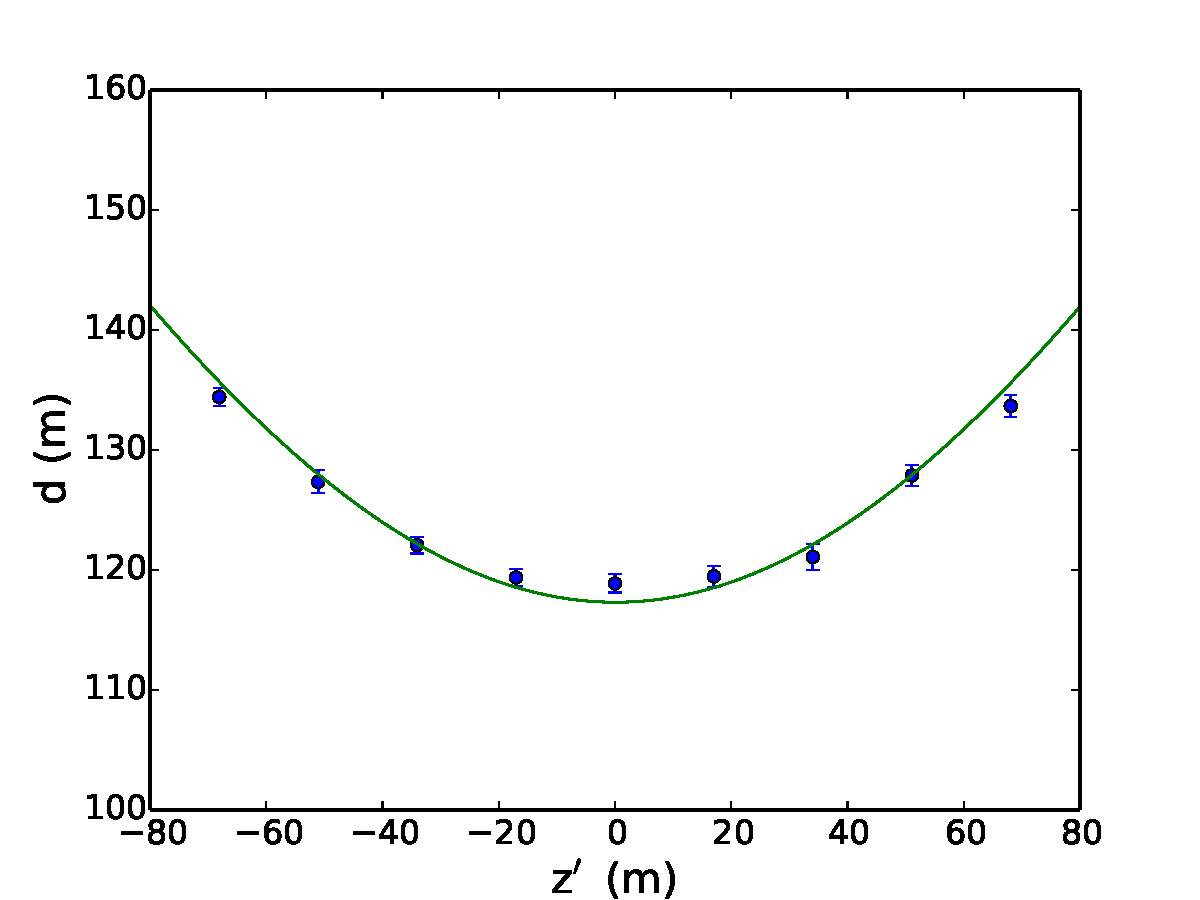
\includegraphics[width=0.5\textwidth]{graphics/geometry/geoparabola.pdf}}
  \subfloat[]{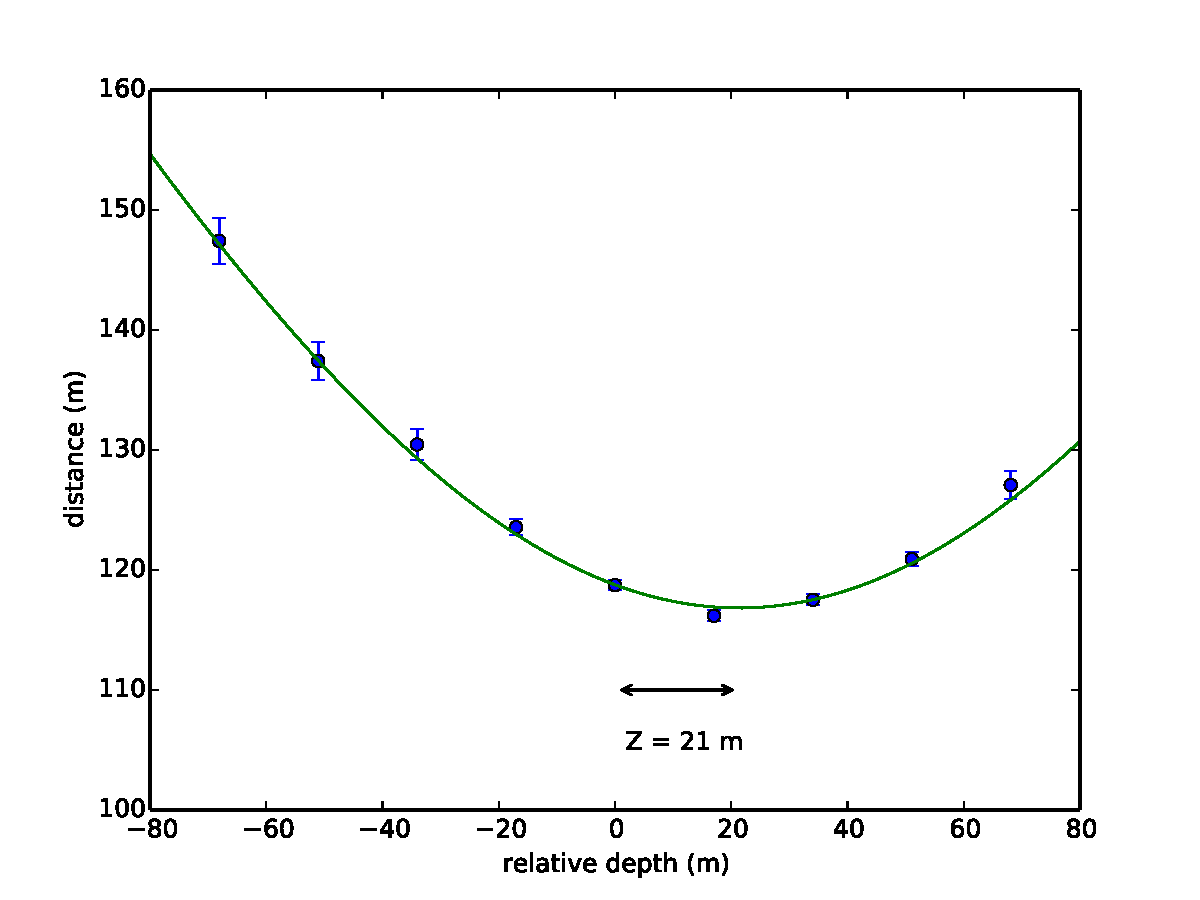
\includegraphics[width=0.5\textwidth]{graphics/geometry/offsetgeoparabola.pdf}}
  \caption{Left: distance $d$ vs.~relative depth $z'$ as measured by flashers for
    two strings that were deployed at nearly the same depth with no
    anomalies during deployment. Right: the same plot for a different pair;
    in this case, the pressure sensor on the flashing string failed during
    deployment.}
  \label{fig:geohyperbola}
\end{figure}


\subsubsection{\label{sec:trilateration}Trilateration Validation of DOM Coordinates}

The Stage 2 geometry assumes that all strings are vertical. The
location data from the drilling process show that the string is not perfectly vertical,
although deviations from the vertical are typically less than 1~m. The
$(x,y)$-coordinates from the drill location data at varying depth were validated on the DeepCore strings
using a trilateration method. In this method, the 5~DOMs closest to the
flasher on each of the three closest strings surrounding the flasher are
selected, and a circle of radius $r = \sqrt{d^2 - (z')^2)}$ is
described around each receiving DOM, where $d$ is the distance between the DOM
and the flasher calculated from the leading edge time of the received
light, and $z'$ is the relative depth of the flashing and receiving
DOMs calculated from the method described above. With 15~circles,
there are 125 possible combinations of three circles which can be used
for trilateration. For each combination, the six intersection points
of the three circles are calculated as shown in
figure~\ref{fig:trilateration}, and the $(x,y)$-position of the flashing DOM 
is taken to be the centroid of the three innermost intersection
points. The final $(x,y)$-position is the average of the values
calculated from each of the 125~combinations of circles. The
error bars on the positions are $1 \sigma$ from a Gaussian fit to all centroid
coordinates; the $x$- and $y$-coordinates are fitted independently. The
measured positions agree with the drill data within the error bars as shown in
figure~\ref{fig:trilateration}. Since the shifts from the nominal
$(x,y)$-coordinates are less than 1~m, and the trilateration measurement is only
practical in a few DeepCore strings where the interstring spacing is 40--70~m, these
corrections were not applied to the IceCube geometry, which still assumes
the vertical string geometry from Stage 2.


\begin{figure}[!ht]
  \captionsetup[subfigure]{labelformat=empty} \centering
  \subfloat[]{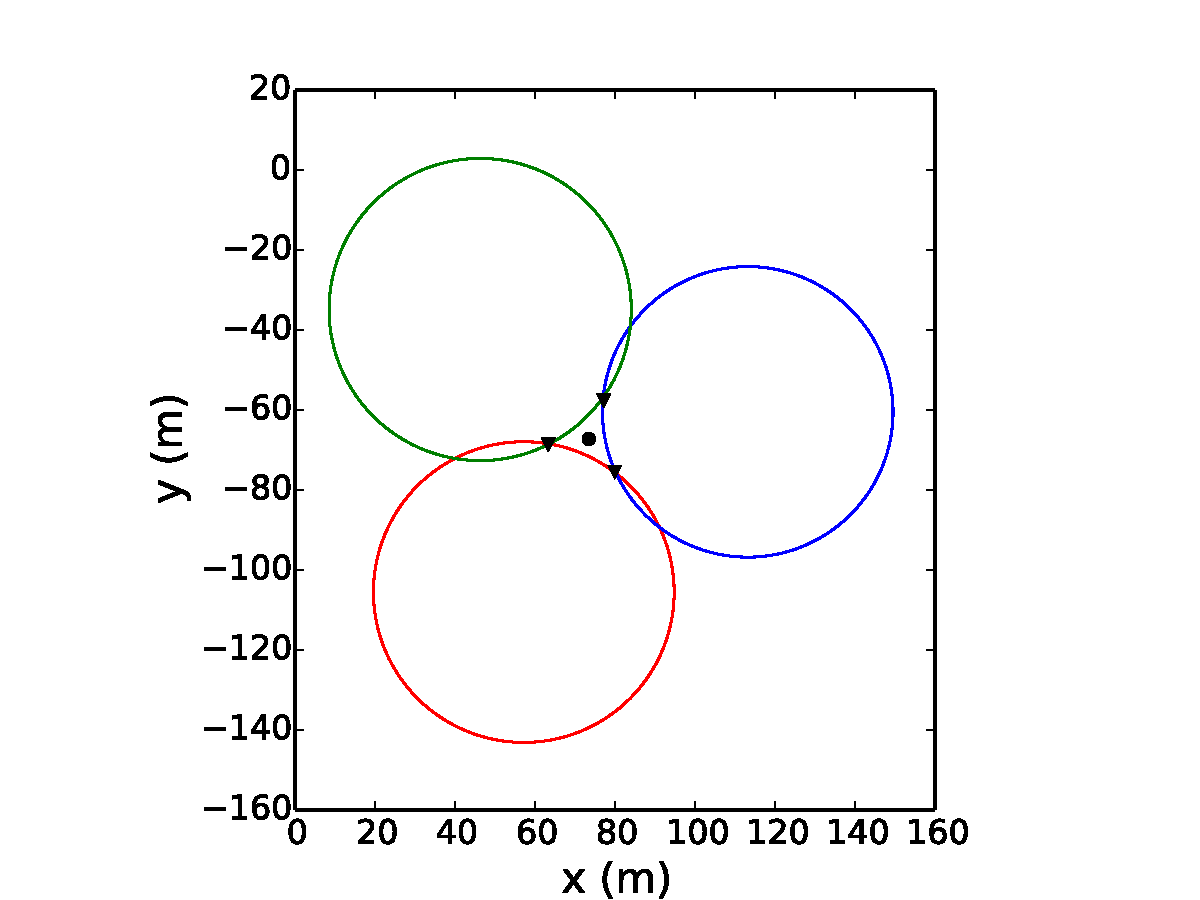
\includegraphics[width=0.48\textwidth]{graphics/geometry/trilat_circles.pdf}}
  \subfloat[]{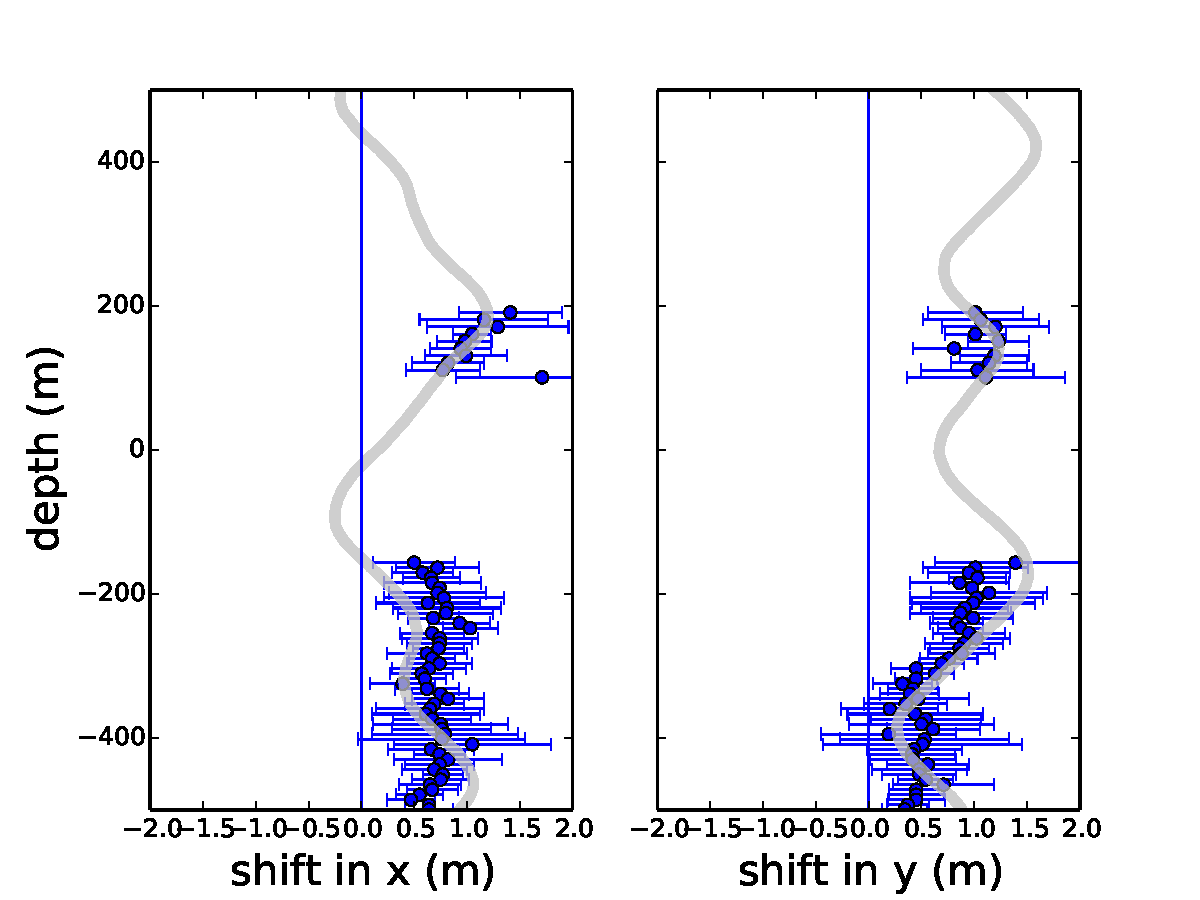
\includegraphics[width=0.48\textwidth]{graphics/geometry/newtrilat85.pdf}}
  \caption{Left: example of three circles drawn around strings
    receiving flasher data from string~80. The inner intersection
    points of the circles are marked with triangles, and the centroid
    of these points, marked with a black dot, is the fitted flasher
    position.  Right: Results of the trilateration fit to String 85, one of
    the DeepCore strings in the center of the detector. The shifts in the
    $x$- and $y$-coordinates are shown as a function of depth, with the drill
    data shown as a gray line.}
  \label{fig:trilateration}
\end{figure}


\subsubsection{Inclinometers}

The stability of the East Antarctic ice sheet is one key feature making it
suitable for a particle physics installation.  However, ice sheets can
deform mechanically under the stress of their own weight.  To measure the
stability of the ice, IceCube installed 50
inclinometers in the deeper sections of the array: two 
electrolytic inclinometers (Applied Geomechanics, Santa Cruz, CA)
housed in $\sim$20-cm-long aluminum pressure modules were installed during
the 2007--2008 season, and 48 micro-electromechanical (MEMS) tilt sensors
(ADIS16209, Analog Devices) were added to DOMs deployed in seasons
2009--2010 and 2010--2011.  This inclinometer array was intended not only for monitoring
detector geometry but also as a unique glaciology experiment that
permits three-dimensional tracking of deep ice flow and evaluation of complex
full-stress models that cannot be effectively tested under laboratory
conditions \cite{pattyn03}.

Figure~\ref{fig:tilt} shows
six years of data from 42 of the DOM-embedded MEMS tilt sensors and
eight years of data from two electrolytic inclinometers. Measurements are
started after 400~days in ice to avoid  
drift due to initial settling of the inclinometers. The electrolytic
inclinometer at \unit[2455]m (86\% ice sheet depth) was 
installed at the bottom of String 68.  For String 45, the drill
descended an additional $\sim$\unit[100]meters in order to deploy an
electrolytic inclinometer attached to a \unit[100]-pound weight at 2540 m
(90\% ice sheet depth) using an extension cable. Data
points are long-term average DOM inclination in degrees per year, with error
bars indicating the standard deviation from trend.  The MEMS sensors have
higher noise than the electrolytic inclinometers, and aging tests have indicated a long-term
drift of $\sim$\numrange[range-phrase = --]{0.02}{0.03}~m/s$^2$, corresponding to
$\sim$\numrange[range-phrase = --]{0.01}{0.02}~degrees per year
\cite{inclinometer_comm}. The MEMS readings are consistent with
$\lesssim$\unit[0.01]degrees of tilt per year with no apparent depth
dependence.  The deep electrolytic sensor 
at \unit[2540]m has shown a persistent \numrange[range-phrase =
  --]{0.07}{0.08} degrees of tilt per year since installation (shear
  of $\tan(0.075^\circ) = 0.0013$
per year).

\begin{figure}[!ht]
	\centering
    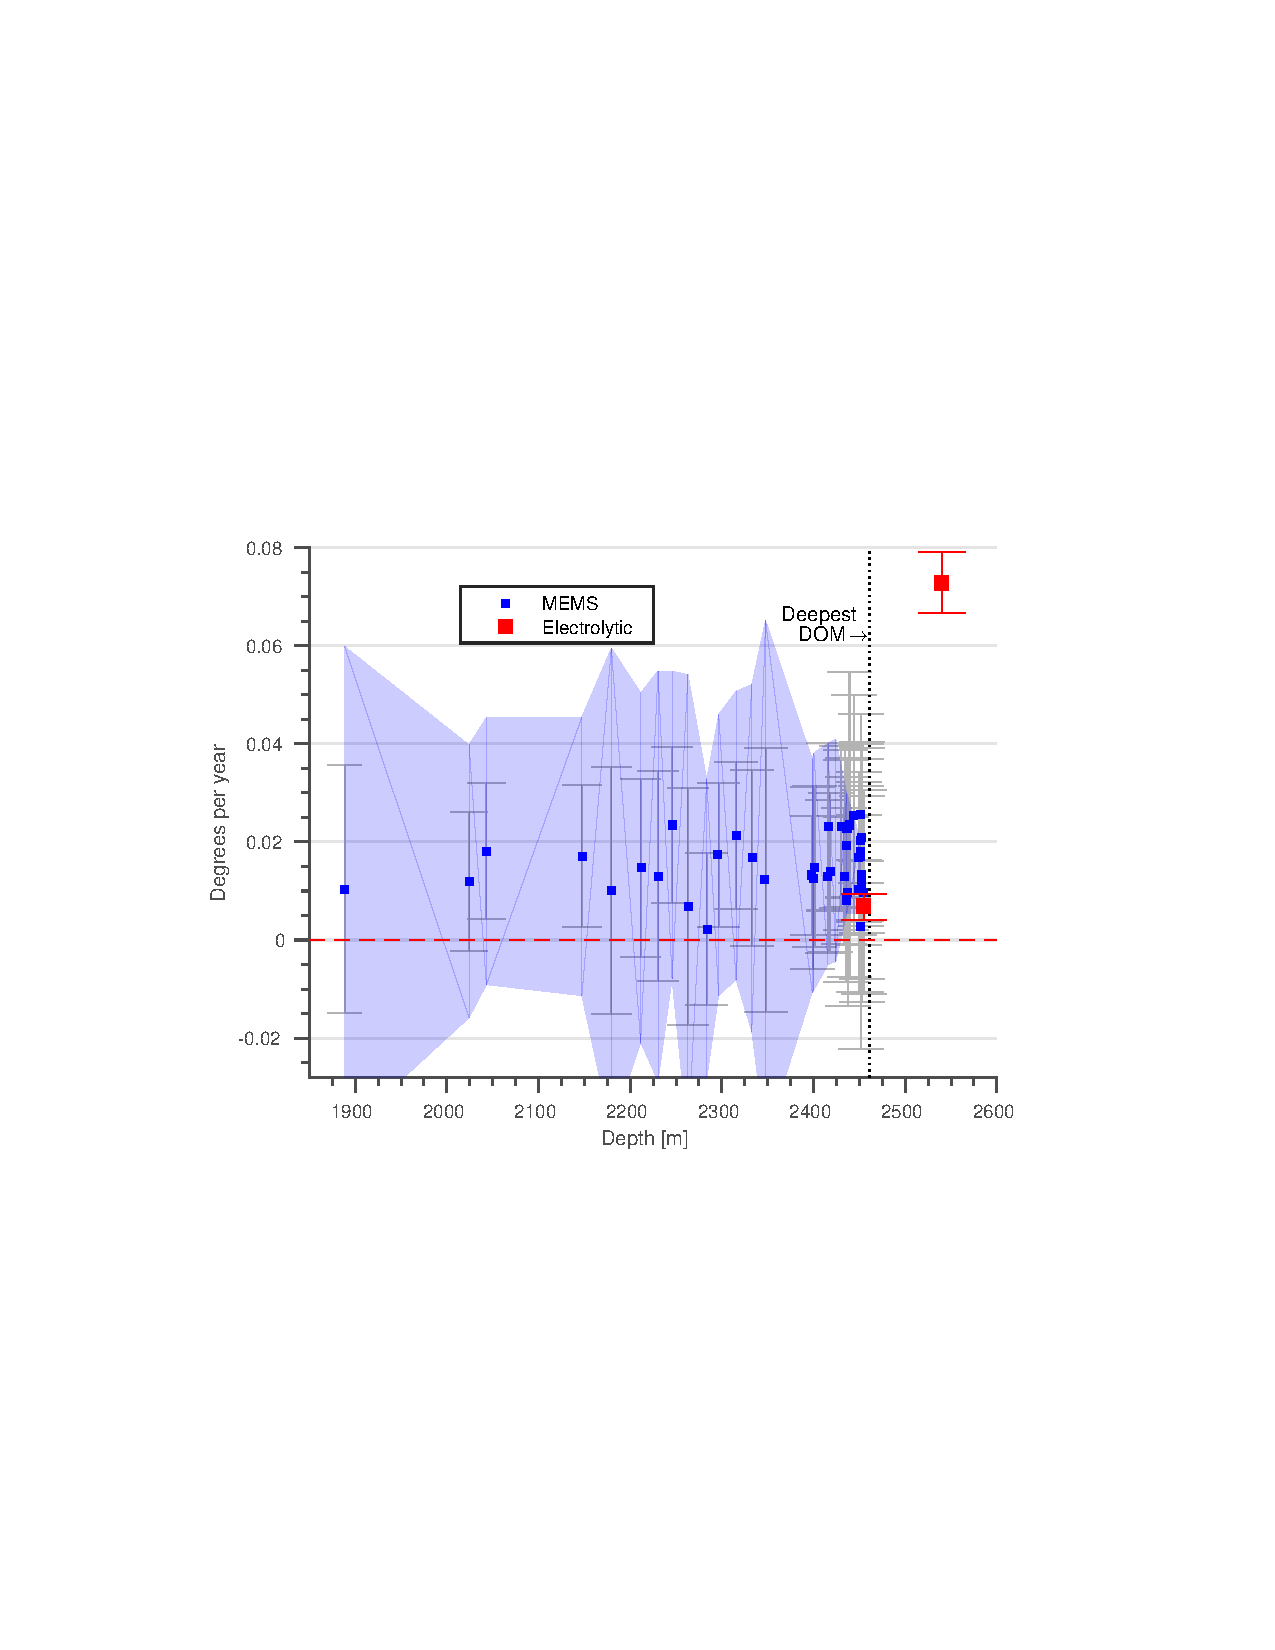
\includegraphics[width=0.7\textwidth]{graphics/geometry/tilt5.pdf}
	\caption{Long term average inclination readings from two electrolytic
      (red) and 42 MEMS (blue) tilt sensors installed in 2007--2011.  Error
      bars show standard deviation from trend; shaded area is MEMS 95\%
      confidence interval in 15 m bins, not including the quoted drift
      from aging tests.  The reading at \unit[2540]m
      indicates increasing strain below the IceCube instrumented volume.}
	\label{fig:tilt}
\end{figure}

In most glaciers at sufficiently great depth, ice strain undergoes a
transition from compression-dominated to shear-dominated with
small-scale folding at centimeter to meter scales~\cite{montagnat14,jansen16}.  This transition depth depends on
temperature \cite{price2002temperature}, grain size, and impurities, and is
associated with a strong single-maximum polycrystalline ice fabric
\cite{cuffey10}.  Tilt sensors within the IceCube instrumented volume, at
depths \SI{<2450}m, show essentially no movement.  Profiles of the
atmospheric dust embedded in the ice measured with dust loggers \cite{I3:dustlogger} show no
indication of folding and appear undisturbed over the full IceCube depth.

\subsection{Hole Ice Imaging Camera}

An imaging camera system, developed at Stockholm University, Sweden, was deployed on String 80 in the final
construction season in order to monitor the freeze-in process and optical
properties of the drill hole.  The system consists of two video cameras
housed in separate glass pressure spheres \SI{5.8}{m} apart, at a
depth of \SI{2455}{m} between the bottom DOM and the string
weights. The cameras can be rotated to point in multiple directions, with some
limitations due to mechanical constraints.  Each
camera is equipped with four LED lamps and three lasers (red, blue, and
green).  Camera heaters, lights, and movement can be controlled remotely
using a dedicated system in the ICL.  

The camera system observed that the drill hole was completely refrozen after
15 days.  The refrozen hole ice consists of a clear outer
layer and a central core of about 16 cm diameter that has much
smaller scattering length than the bulk ice \cite{rongen_vlvnt15}.  The
optical properties of this hole ice are still under active investigation.
No long-term changes have been observed with subsequent camera operations.
